\cotefile{76}
\scanpage{3}

% 1, heading
Complexes \deleted{cellulaires} \inserted{\unsure{côniques|cômiques|coniques}} et \deleted{\unsure{g}}ensembles à opérateurs

% 2, overwritten list, then above it
\[
\begin{aligned}
&\inserted{F_0\quad F_1\qquad F_n}\\
&\deleted{I_0\quad I_1\quad I_n}\qquad\text{ensembles \inserted{(finis?)}}\quad(\unsure{F|I}_\alpha\ \text{ens. des }\alpha\text{-faces})
\end{aligned}
\]

% 3, incidence
\[
\forall\ 0\leq\alpha\leq n-1,\quad I_\alpha\subset F_\alpha\times F_{\alpha+1}\qquad\text{(relation d'incidence)}
\]

% 4, axiom
\uline{Axiome 1} \quad $I_\alpha\to F_{\alpha+1}$ \deleted{et \unsure{$I_\alpha\to F_\alpha$}} est surjectif

% 4, left edge
% margin note written sideways
\margin{\unsure{faudr.t-il|faudrait-il|facultatif} ? \uline{Axiome $1'$} $I_\alpha\to F_\alpha$ surjectif.}

% 5, order
Sur $F_*=\displaystyle\coprod_{0\leq\alpha\leq n}F_\alpha$, on met la relation d'ordre suivante

% 6–9, braced alternatives
\[
\begin{aligned}
\underset{\substack{\rotatebox{90}{$\scriptstyle\ni$}\\F_\alpha}}{x}
<\underset{\substack{\rotatebox{90}{$\scriptstyle\ni$}\\F_\beta}}{y}
\quad\text{ssi}\quad
\left\{\begin{aligned}
&\text{ou bien }x=y\quad(\text{donc }\alpha=\beta)\\
&\text{ou bien }\alpha<\beta,\ \text{et }\exists\ z_\alpha=x\inserted{\in F_\alpha},z_{\alpha\unsure{-|+}1}\in F_{\alpha+1},\ldots,z_{\beta-1}\in F_{\beta-1}\\
&\hspace{2em} z_\beta\deleted{\unsure{\in}}=y\in F_\beta,\quad\text{tels que }\forall\alpha\leq i<\beta,\\
&\hspace{3em}z_i\ \text{et }z_{i+1}\ \text{soient incidents}
\end{aligned}\right.
\end{aligned}
\]

% 10–12, NB
\uline{NB} Le système $(F_\alpha)_{0\leq\alpha\leq n}$ et les $I_\alpha$ $(0\leq\alpha\leq n-1)$ se réconstituent à partir de l'ens. ordonné $F_*$, en prenant

% 13–16, successive minima and long repetition strokes
\[
\begin{aligned}
 F_0&=\text{ens des él. minimaux de }F_*\\
 F_1&=\rule{7em}{.35pt}\quad F_*-F_0\\
 &\unsure{\cdots|\vdots}\\
 F_i&=\rule{7em}{.35pt}\quad F_*-F_0-\ldots-F_{i-1}\qquad(i\leq n)
\end{aligned}
\]

% 13–16, right edge opposite the minima
% slanted
\margin{\uline{NB} Pour une \unsure{partie} de ces considérations, il est \unsure{opportun} de fixer un \unsure{$n$ de référence|ordre inverse}.}

% 17, recovered incidence
\[
 I_\alpha\subset F_\alpha\times F_{\alpha\unsure{-|+}1}\qquad
 I_\alpha=\bigl((x,y)\mid x\in F_\alpha,\ y\in F_{\alpha+1},\ x\leq y\bigr\}
\]

% 18, bracketed line
[Celà marche parceque $I_\alpha\unsure{-|\to} F_{\alpha+1}$ surjectif)

% 19–23, chain condition
Les ens. ordonnés $F_*$ ainsi obtenus sont \unsure{essentiellement} ceux satisfaisant la condition des chaines, et \unsure{.:|.à|où} \inserted{les chaines (= ss-ens. \unsure{totalemt|totalement} ordonnés de $F_{\unsure{\alpha|*}}$) sont de} \deleted{les chaines croissantes \inserted{de ens. ordonnés} d'éléments de $F_*$} longueurs \deleted{maxima} $\leq n$ ($=n$ si on exige $F_n\neq\varnothing$).

% 19–20, left beside chain condition
% slanted
\margin{\uline{vérifier}}

% 24–27, flags
\deleted{\unsure{Ai|Ax}} \uline{Drapeaux} Ce sont par définition les parties \unsure{total.t} ordonnées non vides de $I$. \uline{longueur} d'un drapeau (= son cardinal), type $\in\mathscr P[0,n]$ (c'est une partie \uline{non vide} de $[1,n]$.

% 26–27, lower right
\margin{Ens $\mathscr D(F_*)$ des drapeaux, \unsure{Ordonné|ordonnés} $\subseteq$}

% 28–29, continues at foot
par inclusion, les él. de $F_*$ sont les drapeaux minimaux, la relation $x\leq y$ de $F_*$ signifie \unsure{(équiv.}

% lower left
% archive sheet number: 2
\scanpage{4}

% L1–7, continuation on the left
existe un drapeau majorant $x$ et $y$ ? \unsure{En fait|Il faut|fois} \unsure{donc|dans} \inserted{l'ens ordonné} $F_*$ se récupère via l'ens ordonné des drapeaux (qui a la propriété, entre autres, que tout élément est le sup des éléments minimaux qu'il majore, \inserted{\deleted{\unsure{à is. près avec son ordre}} et des \unsure{paires|l'ens.} des drapeaux \unsure{maj. par} un drapeau} \uuline{cf?).} Drapeaux maximaux\ldots{} Soit $\mathcal A$ l'ens des drapeaux maximaux,

% L1–4, extreme left
% slanted
\margin{au passage à l'ordre inverse près \ldots}

% L8–9, F(x)
\deleted{\unsure{$F_\alpha$}} Pour tout $x\in F_{\deleted{*}\inserted{\alpha}}$, soit $F(x)$ l'ens des $y<x$. \inserted{Il satisfait les m\textsuperscript{es} conditions que $F_*$, avec $n$ remplacé par $\alpha-1$ si $\alpha$\unsure{$\geq 1$|$\neq0$}.} \deleted{On posera l'axiome}

% L10–11, first numbered condition
\uline{Axiome 2} Soit \inserted{$2\leq\alpha\leq n$}, $x_\alpha\in F_\alpha$, $x_{\alpha-2}\in F(x_{\unsure{\alpha|{}}})_{\alpha-2}$. Alors \deleted{\unsure{Il}} le cardinal de l'ens des $y_{\alpha-1}\in F(x_{\unsure{1|\alpha}})_{\alpha-1}$ incidents à $x_{\alpha-2}$ est 2.

% L10–11, left bracket
% slanted
\margin{\unsure{admettre|à mettre|condition} seulement si $n\geq2$}

% L12–13, second condition
\uline{Axiome 3} Soit $x_1\in F_1$, alors le cardinal de l'ens des $y_0\in\deleted{\unsure{F_0,\ x}}\ F(x)_0$ \deleted{incidents à $x$} est 2.

% L12–13, second left bracket
% slanted
\margin{à \unsure{mettre} si $n\geq1$}

% L14–18, maximal flags
\deleted{\unsure{Définissons|Définir|Définition}} Soit alors $\mathcal A$ l'ens des drapeaux maximaux. \deleted{\unsure{de G}} On va introduire sur $\mathcal A$ des opérations $\sigma_\alpha$ $(0\leq\alpha\leq n\deleted{\unsure{\}}}-1)$. Soit $d=(x_0,x_1,\ldots,x_\nu)$ $(\nu\leq n)$ un drapeau maximal, avec $x_i\in F_i$ $(0\leq i\leq\nu)$.

% L19–21, first operator
\[
\begin{aligned}
\sigma_0(d)&=(x'_0,x_1,\ldots,x_\nu)\qquad\deleted{\text{où }x'_0\text{ est}}\ \text{caractérisé par la condition}\\
&\hspace{7em}x'_0\ne x_0\ \big[\text{\uline{et}}\quad(x'_0,x_1,\ldots x_\nu)\ \text{un drapeau}\\
&\hspace{7em}\text{i.e. }x'_0\in F(x_1)_0\big]\qquad\text{cf Axiome 2}
\end{aligned}
\]

% L22–23, remaining operators
\[
\begin{aligned}
1\leq\alpha\leq n-1\quad \sigma_\alpha(d)&=(x_0,\ldots x_{\alpha-1},x'_\alpha,x_{\alpha+1},\ldots)\quad\text{caractérisé par }x'_\alpha\ne x_\alpha\\
&\hspace{8em}\text{\uline{et}}\ \text{que }\sigma_\alpha(d)\ \text{est un drapeau.})
\end{aligned}
\]

% L24–26, optional axiom
Considérons aussi l'axiome (facultatif)

\uline{Axiome $3'$} $\forall x_{n-1}\in F_{n-1}$, le cardinal de l'ens des \deleted{drapeaux} $y\in F_n$ incidents à $x_{n-1}$ est 2.

% L25–27, outer left bracket
% slanted
\margin{pour $n\geq1$ fixé}

% L27–28, last operator
On pose alors
\[
\sigma_n(d)=(x_0,\ldots,x_{n-1},x'_n),\quad \deleted{\text{où }x'_n\text{ est le}}\ \inserted{\text{caractérisé par }x'_n\ne x_n\quad\text{\unsure{(et\ldots)|(etc.\ldots)}}}
\]

% L29–30, foot of left column
\uline{NB} Les $F(x)$ (où $x\in F_\alpha$) satisfont les axiomes $1,2,3$, \uline{et $4$} avec $n$ remplacé par $\alpha-1$\ldots

% R1–3, head of right column
On va voir maintenant que (moyennant les axiomes 1, $1'$, 2, \unsure{3, $3'$|$2'$, 3} \inserted{et un axiome 4 plus bas}) l'ens à opérateurs $\mathcal A$ permet de \uline{reconstituer} $F_*$ (donc $(F_\alpha),(I_\alpha)$\ldots).

% R4–6, commutations
\deleted{On \unsure{vérifie|a évidemment}} \deleted{Les} Mais donnons d'abord les relations de commutation évidentes
\[
 \sigma_\alpha\sigma_\beta=\sigma_\beta\sigma_\alpha\qquad\text{si }|\beta-\alpha|\ne1\quad\text{i.e. }\alpha,\beta\ \text{non consécutifs.}
\]

% R7–11, group and subgroup
Soit $G_n$ le groupe engendré par les \deleted{\unsure{rela\textsuperscript{ts}|relations}} gén. $\sigma_\alpha$ $(0\leq\alpha\leq n)$ avec les relations précédentes. $\mathcal A$ est un $G_n$-ensemble. Les $\sigma_\alpha$ y opèrent sans pt fixe. Soit $G_n^{(\alpha)}$ \inserted{$(0\leq\alpha\leq n)$} le sous-groupe de $G_n$ engendré par les $\sigma_\beta$ avec $\beta\ne\alpha$.

% R12–13, orbit map
On a évidemment
\[
 \mathcal A/G_n^{(\alpha)}\longrightarrow F_\alpha\qquad\unsure{(\text{si }\alpha\leq n-1)|(0\leq\alpha\leq n-1)}
\]

% R14–20, fourth axiom with justification
\deleted{\unsure{Proposition}} \inserted{\uline{Axiome 4}} Cette application est bijective. (La surjectivité est claire \inserted{par l'axiome 1}. Pour la bijectivité, il suffit de voir que si $d=(x_0,\ldots x_n)$, $d'=(\unsure{x_0|x'_0},\ldots x'_n)$ sont des él\textsuperscript{ts} avec \deleted{$d,d'$ \illegible{1}}, $x_\alpha=x'_\alpha$, alors \deleted{\unsure{op}} on peut passer de $d$ à $d'$ en appliquant successiv\textsuperscript{mt} des transformations $\sigma_\beta$ avec $\beta\ne\alpha$.

% R14–15, in the gutter
% slanted
\margin{le \unsure{rendre} naturel}

% R21–24, a general type
Plus généralement, soit $\delta\subset[0,n]$, \inserted{$\delta\ne\varnothing$} et considérons le sous-groupe $G_n^{(\delta)}$ de $G_n$, engendré par les $\sigma_i$ avec $i\in\complement_{[0,n]}\delta$, Alors on a

% R25, lower right
\[
 \mathcal A/G_n^{(\unsure{\alpha|\delta})}\unsure{-|\to}\mathcal A_\delta\quad\text{(drapeaux de type }\delta\text{)}
\]

% R26–28, final question
et on voudra que ce soit bijectif (est-ce une conséquence de l'axiome 4 et des précédents?).

% bottom left
% archive sheet number: 3
\scanpage{5}

% 1–8, inclusion and incidence
Ceci dit, les relations d'inclusion naturelles entre les $G_n^\delta$ ($G_n^\delta\subset G_n^{\delta'}$ pour $\delta'\subset\delta$) définissent les relations d'incidence \inserted{(= \unsure{prolonger et restreindre|prolongement et restriction|relations d'inclusion})} entre drapeaux de types \deleted{\unsure{$\delta$}} divers. On reconstitue ainsi l'ens ordonné des drapeaux des divers types $\delta$, et par là l'ens des $F_\alpha$ (drapeaux minimaux) et leurs relations d'incidence\ldots.

% 9, transition
De façon précise :

% 10–14, proposition
\uline{Prop} Le foncteur $(F_*)\unsure{\mapsto|\vdash}(\mathcal A)$ des complexes cellulaires satisfaisant les conditions $1,1',2,2',3,4$ (renforcé ?) vers les ens à groupe d'opérateurs $G_n$, est \uline{pl. fidèle}.

% 15–16, essential image
Il faudrait déterminer l'image essentielle.

% after 16, separator
\figure{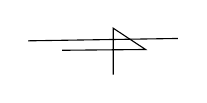
\begin{tikzpicture}[x=1cm,y=1cm]\draw (-.95,0) -- (.95,.03); \draw (-.52,-.12) -- (.54,-.11) -- (.13,.16) -- (.13,-.43);\end{tikzpicture}}

% 17–21, geometric realization
Réalisation géom. d'un complexe $F_{\unsure{\alpha|*}}$ (satisfaisant \unsure{les deux axiomes|le seul axiome} 1) : c'est par définition la réalisation géométrique de la triangulation combinatoire définie par l'ens des parties \inserted{(finies)} tot\textsuperscript{t} ordonnées de \deleted{\unsure{$F$}}$F_*$.

% lower left
% archive sheet number: 4
\scanpage{6}

% top, automorphisms and vertical extension
\diagram{\begin{tikzcd}[ampersand replacement=\&,column sep=small,row sep=small]
\& \& 1\\
1\arrow[r] \& {\text{\uline{Aut}}(X,\mathrm{id}_{\partial X})}\arrow[r] \& \mathrm{Aut}(X)\arrow[u]\arrow[r,dash] \& \mathrm{Aut}(\partial X)\arrow[r,dash] \& 1\\
\& {}\arrow[r] \& \widetilde{\mathrm{Aut}}(X)\arrow[u]\\
\& \& \mathbb Z^I\arrow[u]\\
\& \&1\arrow[u]
\end{tikzcd}}

% upper left, boundary and projection
\diagram{\begin{tikzcd}[ampersand replacement=\&,row sep=small,column sep=small]
\& \widetilde{\partial X}\arrow[d,"p"]\\
 X\&\partial X\arrow[l,hook]
\end{tikzcd}}

% upper middle, pairs of automorphisms
\[
\begin{aligned}
\underset{\substack{\rotatebox{90}{$\scriptstyle\subset$}\\
\mathrm{Aut}(X)\times\mathrm{Aut}(\widetilde{\partial X})}}{\widetilde{\mathrm{Aut}}(\overset{\unsure{\prime\prime|i|\ast}}{X})}
=\bigl\{(u,\widetilde v)\mid u\in\mathrm{Aut}(X),\widetilde v\in\mathrm{Aut}(\widetilde{\partial X}),\
(u\mathbin{\upharpoonright}\partial X)\circ p=p\circ\widetilde v
\end{aligned}
\]

% middle, grid with dashed diagonal
\diagram{\begin{tikzcd}[ampersand replacement=\&,column sep=small,row sep=small,execute at end picture={\draw[thin] ([xshift=-4pt,yshift=3pt]\tikzcdmatrixname-1-3.north west) -- ([xshift=2pt]\tikzcdmatrixname-5-3.south east);}]
\&1\&1\\
1\arrow[r,dash]\& S\mathcal A(X)\arrow[u]\arrow[r]\arrow[dr,dashed]\&\mathcal A(X)\arrow[u]\arrow[r]\&\mathcal A(\partial X)\arrow[r,dash]\&1\\
1\arrow[r,dash]\& \underset{S\mathcal A(X)\times\mathbb Z^I}{S\widetilde{\mathcal A}(X)}\arrow[u]\arrow[r]\&\widetilde{\mathcal A}(X)\arrow[u]\arrow[r]\&\mathcal A(\widetilde{\partial X})\arrow[u,"\unsure{1|\wr}"]\arrow[r,dash]\&1\\
1\arrow[r,dash]\&\mathbb Z^I\arrow[u]\arrow[r,Rightarrow]\&\mathbb Z^I\arrow[u]\arrow[r,dash]\&1\arrow[u]\arrow[r,dash]\&1\\
\&1\arrow[u]\&1\arrow[u]
\end{tikzcd}}

% middle grid, far right
\margin{$I=\pi_{0}(\partial X)$}

% bottom, grid with quotients
\diagram{\begin{tikzcd}[ampersand replacement=\&,column sep=small,row sep=small,execute at end picture={\draw[thin] (\tikzcdmatrixname-1-3.south east) -- (\tikzcdmatrixname-5-4.south east);}]
\&1\&\unsure{1|\wedge}\&1\\
1\arrow[r,dash]\&ST(X)\arrow[u]\arrow[r]\arrow[dr,dashed]\&\mathcal A(X)/S\mathcal A^\circ(X)\arrow[u]\arrow[r,dash]\&\mathcal A(\partial X)\arrow[u]\arrow[r,dash]\&1\\
1\arrow[r]\&\underset{\unsure{\simeq}ST(X)\times\mathbb Z^I}{S\widetilde T(X)}\arrow[u]\arrow[r]\&\widetilde{\mathcal A}(X)/S\unsure{\mathcal A^\circ|\mathcal M}(X)\arrow[u]\arrow[r,dash]\&\mathcal M\unsure{\partial X)|(\partial X)|(\widetilde{\partial X})}\arrow[u,"\unsure{\sim|2|\wr}"]\arrow[r,dash]\&1\\
1\arrow[r,dash]\&\mathbb Z^I\arrow[u]\arrow[r,Rightarrow]\&\mathbb Z^I\arrow[u]\arrow[r]\&\unsure{1|?}\arrow[u]\arrow[r,dash]\&1\\
\&1\arrow[u]\&1\arrow[u]\&\deleted{\unsure{1|?}}1\arrow[u]
\end{tikzcd}}

% oblique line
% One diagonal pen stroke crosses the working from below the first row to the foot of the last grid.

% lower left
% archive sheet number: 5
\scanpage{7}

% 1–7, realization of elements
Les éléments du $F_\alpha$ se réalisent comme parties \inserted{(à structure \unsure{cônique|conique|coniques})} de $|F_*|$ [\unsure{la ré.|la ré\textsuperscript{o}|associé} à $x\in F_{\unsure{n|\alpha}}$ correspond la réunion des simplexes réalisations des simpl. \deleted{fermés} \inserted{\unsure{corresp|ouverts}} d'élément $\leq x$], la relation d'incidence devient l'inclusion --- il y a une équivalence de catégories (\deleted{\unsure{top.}} d'objets top. versus objets combinatoires) à dégager.

% 8–10, proposition beside vertical rule
\uline{Prop} Si $|F_*|$ est une variété top. \inserted{\unsure{pure|petit|pointée}} de dim $n$, alors $(F_\alpha)$ satisfait les conditions $\deleted{\unsure{I}}1,1',2,2',3,4$\ldots

% 10–14, more precise criterion
[Plus précisément, pour que $(F_*)$ soit une variété top. de dim $n$, il f. et s. que $(F_*)$ satisfasse $1,1',2,2',3,3',4$, \uline{et} que $\forall x\in F_\alpha$, \inserted{$(\alpha\geq3)$}, la réalisation géom. de $F(x)$ soit une sphère

% 14–18, nested qualification
[en fait, \deleted{\unsure{et}} si on a l'hyp. de Poincaré, il suffit d'exiger que \deleted{pour $\alpha\geq\unsure{3,4|3?|3}$}, $|F(x)|$ soit simplement connexe et \deleted{ait} \inserted{pour $\alpha\geq5$, il ait de plus} l'homologie d'une sphère de m\textsuperscript{e} dimension.

% after 18, divider
\figure{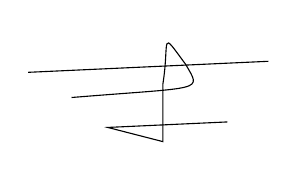
\begin{tikzpicture}[x=1cm,y=1cm]\draw (-1.55,.3)--(1.5,.44); \draw (-1,-.02).. controls (.7,.12) and (.65,.05) ..(.45,.4).. controls (.11,.86) and (.25,.72) ..(.16,.15)--(.16,-.58)--(-.54,-.4)--(.98,-.33);\end{tikzpicture}}

% 19–20, filtered space
Soit $X$ un espace top. \inserted{(\unsure{compact ?|compact ??})} filtré par
\[
 X_0\subset X_1\subset\ldots\subset X_n=X.
\]
\deleted{On suppose \unsure{$X$} est} \inserted{$X$ \unsure{var.} de dim $n$}

% 21–23, successive differences
que $\forall i=0,\ldots,n-1$, la \uline{différence} de $X_{i+1}$ suiv\textsuperscript{ant} $X_i$ est \deleted{une variété} \inserted{homéomorphe} à \deleted{boule de di\unsure{m}} \inserted{une} réunion de boules $D^{i+1}$.

% 23–26, flags of the filtration
Soit $\mathcal A$ l'ens des ``drapeaux'' relatifs à cette filtration (à définir avec soin). On a alors une op. de $G_{n\unsure{(+1)|+1}}$ (\deleted{\unsure{resp. =}} $G_n$ si $X$ \unsure{de la variété|déjà variété|variété} top. de dim $n$)

% lower left
% archive sheet number: 6
\scanpage{8}

% 1, continuation
avec les $\sigma_i$ opérant ss pt fixe.

% 2–5, proposition
\uline{Prop} le foncteur de la catégorie isotopique des \inserted{variétés de dim $n$} $X$ filtrés comme dessus, vers les $G_n$ ensembles finis (où les $\sigma_i$ opèrent ss pt fixe) est \uline{pl. fidèle}.

% 6–11, essential image
Déterminer l'image essentielle (\unsure{admettre|mettre|moyennant} l'hyp. de Poincaré au besoin) et montrer qu'elle est plus grande que celle correspondant aux complexes cellulaires se réalisant suivant une variété topologique\ldots.

% 12–16, combinatorial variety
\uline{$n$-Variété combinatoire} \inserted{\uline{finie}}, définie par un ens \inserted{fini} $D_n$ muni d'autom. invol. sans pts fixes $\sigma_i$ $(0\leq i\leq n)$ tels que deux $\sigma_i$ \unsure{:} non consécutifs commutent --- i.e. $D_n$ est un ens. à op. sous $G_n$, avec les $\sigma_i$ $(0\leq i\leq n)$ op. sans pts fixes.

% 17–20, combinatorial complex
\uline{$n$-complexe combinatoire} \uline{fini} Donné par un système $D_n,D_{n-1},\ldots,D_1,\underset{\substack{\downarrow\\\text{``spécial''}}}{D_0}$ d'ens \inserted{finis}, chaque \inserted{$D_i\ (1\leq i\leq n)$} étant un \deleted{\unsure{$D_i$}} $G_{i-1}$-ensemble (\deleted{\unsure{à él\textsuperscript{ts}|i.e.}} les gén. $\sigma_\alpha$ \unsure{op.} sans pts fixes) et des applications

% 21, sequence of applications
\[
 D_n\to D_{n-1}\longrightarrow D_{n-2}\longrightarrow\ldots\longrightarrow D_1\longrightarrow D_0
\]

% 22–23, compatibility, continues
telles que $\forall\,2\leq i\leq n$, $D_i\to D_{i-1}$ soit un $G_{i-2}$-morphisme, et que pour $\deleted{\unsure{2\leq j\geq{}|0\leq j\leq{}}}i\geq j+2\geq j\geq0$,

% lower left
% archive sheet number: 7
\scanpage{9}

% 1–3, continuation
l'application composée $D_i\unsure{-|\to}D_j$ (qui est un $G_{j-1}$-morphisme) soit invar\textsuperscript{te} par $\sigma_{i-1},\ldots,\sigma_{j+1}$

% 4, equivalence
\uline{$n$-variété combinatoire} $\leftrightarrow G_n$-ens. $D_n$

% 5–6, boundary
Si $0\leq i\leq n$, le \deleted{\unsure{$(i-1)$-découpé|décomp.}} \inserted{bord \unsure{du le|de la|du} \unsure{$i$-découpage|$i$-découpé|$i$-décomp.}} $\delta_{i-1}$ \inserted{$\partial(\unsure{\mathrm{Déc}|\mathrm{déc}}(X_i/X_{i-1})$} est une $i-1$ variété combinatoire qui est

% 7–11, successive boundary objects
\[
\begin{aligned}
\delta_{n-1}&=(D_n\,;\sigma_0,\ldots\sigma_{n-1})\\
\delta_{n-2}&=(D_n/\sigma_n\,;\sigma_0,\ldots,\sigma_{n-2})\\
\delta_{n-3}&=(D_n/(\sigma_n,\sigma_{n-1})\,;\sigma_0,\ldots,\sigma_{n-3})\\
&\ldots\\
\delta_{i-1}&=(D_n/(\sigma_n,\ldots\sigma_{i+1})\,;\sigma_0,\ldots\sigma_{i-1})
\end{aligned}
\]

% 12–13, beginning of crossed block
\deleted{On définit par réc. sur $n$ la cat. $\mathcal C_n$ des $n$-\deleted{\unsure{complexes}}\inserted{cartes} combinatoires, \deleted{en posant} \inserted{(finies) et foncteur $i_n:\mathcal C_n\to\mathcal V_n$}}

% 13–14, at right of crossed block
\margin{\deleted{$n$-var. comb.}}

% 14–18, crossed definitions
\[
\begin{aligned}
&\deleted{\mathcal C_0=\deleted{0\text{-complexes}}\inserted{0\text{-\unsure{espaces|sphères}}}\ \text{comb.}=\text{ens finis}}\\
&\deleted{\ldots}\\
&\deleted{\mathcal C_n=\inserted{\text{cat. des}}\ \{X_{n-1},S_{n-1},p\}\quad\text{où}\quad X_{n-1}\in\operatorname{Ob}\mathcal C_{n-1}}\\
&\hspace{13em}\deleted{S_{n-1}\in\operatorname{Ob}\unsure{\mathcal V_{n-2}|\mathcal V_{n-1}},\ \deleted{\text{\unsure{convient}}}}\\
&\hspace{13em}\deleted{\varphi:i_{n-1}(\unsure{S_{n-1}|b_{n-1}})\to X_{n-1}}
\end{aligned}
\]

% 19–21, crossed functor and unfinished expression
\deleted{$i_n:\unsure{\mathcal V_n|\mathcal C_n}\to\mathcal C_n$ défini par}
\[
 \deleted{i_n(\underset{\substack{\searrow\\G_n\text{-ens.}}}{D_n})=(}
\]

% lower left
% archive sheet number: 8
\scanpage{10}

% 1, title
\uline{\deleted{Complexes}\inserted{Cartes} coniques}, \uline{\deleted{complexes}\inserted{cartes} \deleted{cellulaires}}, et \uline{ens. à opérateurs}.

% 2–5, filtered space
Une \uline{$n$-carte conique} \inserted{(finie)} est un espace top. $X$ compact, muni d'une filtration croissante \inserted{par des parties \uline{fermées}}
\[
 X_0\subset X_1\subset\ldots\subset X_{n-1}\subset X_n=X
\]
telles que

% 6, first condition
a) $X_0$ fini (i.e. discret)

% 7–12, second condition
b) pour $1\leq i\leq n$, \inserted{soit $\bar Z_i={}$} $\operatorname{Déc}(X_i/X_{i-1})\deleted{=\bar Z_i}$ (découpage de $X_i$ suivant $X_{i-1}$), $\dot Z_i=\bar Z_i\mid X_{i-1}$ (NB on a $Z_i\to X_i$, induisant un isom. $\bar Z_i-\dot Z_i\longrightarrow X_i-X_{i-1}$), alors \deleted{les composantes} \inserted{$\bar Z_i$ a un n\textsuperscript{b} \uline{fini} de comp. connexes,} et chacune $\bar Z_i^\alpha$ est \unsure{isom.|hom.|homéom.} au cône sur $\dot Z_i^\alpha=\bar Z_i^\alpha\cap\dot Z_i$ (et $\dot Z_i^\alpha\ne\varnothing$)

% 13, finite morphism
c) $\dot Z_i\to X_{i-1}$ est un morphisme fini, \deleted{dont l'image}

% 14, fourth condition and interline
\deleted{\unsure{c)}} d) La filtration de $X$ est équisingulière \inserted{[$\Leftrightarrow\bar Z_i\to X_{\unsure{j|i}-1}$ est \unsure{constant|constante} sur \unsure{les|une} \unsure{comp.|c.c.} de $X_j-X_{j-1}$ $(j\leq i-1)$]}

% 14–16, right of examples
\margin{d) \unsure{Soit|Soit l'} image \inserted{$X'_{i-1}$} de $\bar Z_i$ ds $X_{i-1}$ \deleted{\unsure{$X'_i$}} Alors $X'_{i-1}=\overline{X'_{i-1}\cap\complement X_{i-2}}$}

% 15–16, small dimensions
Cas $n=0$ : espaces finis discrets

Cas $n=1$ : \qquad $\underbrace{X=X_1}_{\text{cpt}}\supset X_0$.

% lower left, decomposition in dimension one
\diagram{\begin{tikzcd}[ampersand replacement=\&,row sep=small,column sep=tiny]
\dot Z_1\arrow[d]\&{}=\coprod_\alpha\dot Z_1^\alpha\\
X_0
\end{tikzcd}}

% lower right, dimensions zero to three
\diagram{\begin{tikzcd}[ampersand replacement=\&,row sep=small,column sep=1ex]
\overset{\deleted{\unsure{x}}}{\dot x_0}\in\overset{\deleted{\unsure{x}}}{y_1}\&\&\overset{\deleted{\unsure{x}}}{\dot x_1}\quad y_2\\
\dot Z_1\arrow[d]\arrow[r,phantom,"\subset" description]\&\overset{\deleted{\unsure{m}}}{\bar Z_1}\arrow[d]\&\dot Z_2\arrow[dl]\arrow[r,phantom,"\subset" description]\&\bar Z_2\arrow[d]\&\dot Z_3\arrow[dl]\arrow[r,phantom,"\subset" description]\&\bar Z_3\arrow[d]\\
 X_0\arrow[r,phantom,"\subset" description]\&X_1\arrow[rr,phantom,"\subset" description]\&\&X_2\arrow[rr,phantom,"\subset" description]\&\&X_3\\
 x_0\arrow[r,phantom,"\subset" description]\&x_1\arrow[rr,phantom,"\subset" description]\&\&x_2\arrow[rr,phantom,"\subset" description]\&\&x_3
\end{tikzcd}}

% lower left, loop with a point
\figure{
\begin{tikzpicture}[scale=.65]\draw (0,0)..controls (.2,.8) and (1.2,1.15)..(1.44,.66)..controls (1.55,.33) and (.45,-.16)..(0,0);\fill (0,0) circle (.055);\end{tikzpicture}}

% lower left, sloping interval
\figure{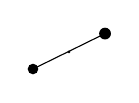
\begin{tikzpicture}[scale=.75]\draw (0,0)--(1.22,.6);\fill (0,0) circle (.09) (.61,.29) circle (.025) (1.22,.6) circle (.1);\end{tikzpicture}}

% lower left, nearly horizontal interval
\figure{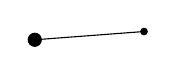
\begin{tikzpicture}[scale=.75]\draw (0,0)--(1.85,.14);\fill (0,0) circle (.12) (1.85,.14) circle (.065);\end{tikzpicture}}

% lower right, general ranks
\diagram{\begin{tikzcd}[ampersand replacement=\&,row sep=small,column sep=1ex]
\dot x_{i+1}\&\dot Z_{i+1}\arrow[d]\arrow[r,phantom,"\subset" description]\& Z_{i+1}\arrow[d,dash]\&\dot Z_{i+2}\arrow[dl]\arrow[r,phantom,"\subset" description]\&\bar Z_{i+2}\arrow[d]\\
X_{i-1}\arrow[r,phantom,"\subset" description]\&X_i\arrow[r,phantom,"\subset" description]\& X_{i+1}\arrow[rr,phantom,"\subset" description]\&\&X_{i+2}\\
\&x_i\&\&\&x_{i+2}
\end{tikzcd}}

% lower left, three branches
\figure{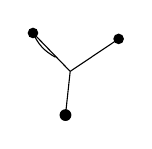
\begin{tikzpicture}[scale=.75]\draw (-.63,.65)--(0,0)--(.82,.55) (0,0)--(-.08,-.74); \draw (-.63,.65) to[bend right=18](-.25,.24); \fill (-.63,.65) circle(.09) (.82,.55) circle(.09) (-.08,-.74) circle(.1);\end{tikzpicture}}

% beside three branches, short stroke
\figure{
\begin{tikzpicture}[scale=.7]\draw[line width=1.2pt](0,0)--(.45,.47);\fill(.45,.47)circle(.055);\end{tikzpicture}}

% bottom left, curved arcs
\figure{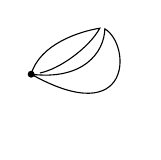
\begin{tikzpicture}[scale=.8]\draw (0,0)..controls (.14,.48) and (.77,.68)..(1.09,.73)..controls (.92,.42) and (.45,.08)..(.14,.02); \draw (0,0)..controls (.82,-.1) and (1.16,.34)..(1.17,.72)..controls (1.59,.47) and (1.61,-.9)..(0,0);\fill (0,0)circle(.055);\end{tikzpicture}}

% bottom middle, sector and rays
\figure{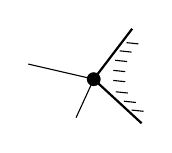
\begin{tikzpicture}[scale=.8]\draw[thick](.61,.8)--(0,0)--(.76,-.7); \draw (-1.04,.24)--(0,0)--(-.28,-.61); \fill(0,0)circle(.11); \foreach \x/\y in {.52/.58,.41/.45,.34/.3,.31/.14,.31/-.02,.35/-.2,.48/-.35,.6/-.49}{\draw (\x,\y)--++(.19,-.02);}\end{tikzpicture}}

% bottom right, restricted terms
\diagram{\begin{tikzcd}[ampersand replacement=\&,row sep=small,column sep=small]
{\dot Z_{i+2}|X_{i-1}}\arrow[d,dash]\arrow[r,phantom,"\subset" description]\&{\dot Z_{i+2}|X_i}\arrow[d]\arrow[r,dash]\&\bar Z_{i+2}\arrow[d]\\
X_{i-1}\arrow[r,phantom,"\subset" description]\&X_i\arrow[r,phantom,"\subset" description]\&X_{i+2}
\end{tikzcd}}

% bottom left, dimension-one square
\diagram{\begin{tikzcd}[ampersand replacement=\&,row sep=tiny,column sep=small]
\dot Z_1\arrow[d]\arrow[r,phantom,"\subset" description]\&\bar Z_1\arrow[d]\\
X_0\arrow[r,phantom,"\subset" description]\&X_1
\end{tikzcd}}

% lower left
% archive sheet number: 9
\scanpage{12}

% 1, opening
Ens ordonné des cellules \deleted{\unsure{f.}} ouv. $X_i$

% 2–3, two lines of X terms
\diagram{\begin{tikzcd}[ampersand replacement=\&,row sep=tiny]
\bar X_{i-1}\arrow[d,dash]\\ X_{i-1}\quad X_i\&X_i
\end{tikzcd}}

% 4, heading
Géométrie des drapeaux de dim $\leq n$

% 5, examples
$D_0$ \uline{Ex} \qquad $n=0$\qquad $D_0$

% 6–7, first fork
\diagram{\begin{tikzcd}[ampersand replacement=\&,row sep=small,column sep=small]
n=1\&\&D_{01}\arrow[dl]\arrow[dr,"\text{\uline{épi} !!}"]\\
\&D_0\&\&D_1
\end{tikzcd}}

% 7–8, scratched repetition to the left
$\deleted{\bar X_{i-1}}\quad\deleted{X_{i-1}\ X_i}$ \quad $n=2$

% 8–10, three levels below the long line
\diagram{\begin{tikzcd}[ampersand replacement=\&,column sep=0.4em,row sep=small]
\&\& D_{012}\arrow[dl,dash]\arrow[d,dash]\arrow[dr,"\text{épi}",dash]\\
\&D_{01}\arrow[dl,dash]\arrow[dr,"\text{épi}"']\&D_{02}\arrow[dll,dash]\arrow[drr,dash]\&D_{12}\arrow[dl,dash]\arrow[dr,"\text{épi}",dash]\\
 D_0\&\&D_1\&\&D_2
\end{tikzcd}}

% 8–10, right of the triangle
$D_{01\ldots i}\to D_I$ \uuline{épi} si $i=\operatorname{Sup} I$ i.e. $i\in I\subset[0,i]$

% 11, central label
$D_I$

% 12–15, central fork with F labels
\diagram{\begin{tikzcd}[ampersand replacement=\&,row sep=small,column sep=.5em]
\&\&D_{012}(F)\arrow[ddl,dash]\arrow[d]\arrow[dr,"\text{épi}"]\\
\&\&D_{02}(F)\arrow[ddll,dash,bend left=15]\arrow[ddrr,dash,bend right=10]\&D_{12}(F)\arrow[ddl,bend right=12]\arrow[ddr,"\unsure{e}"]\\
\&D_{01}\arrow[dl,dash]\arrow[dr]\\
D_0\&\&D_1\&\&\unsure{\{M\}|\{m\}|\{1\}}
\end{tikzcd}}

% 12–14, separate square at right
\diagram{\begin{tikzcd}[ampersand replacement=\&,row sep=small,column sep=small]
D_{012}\arrow[r]\arrow[d]\&D_{12}\arrow[d,dash]\\
D_{02}\arrow[r]\&D_2
\end{tikzcd}}

% 14–16, left-hand scratch
\diagram{\begin{tikzcd}[ampersand replacement=\&,row sep=tiny,column sep=small]
j\quad j{+}1\&D_{123}\arrow[d]\\
\deleted{D_{j\ldots j}}\&D_{13}\\
\&\overline{D_{13}}
\end{tikzcd}}

% 15–16, central bracket
\figure{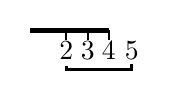
\begin{tikzpicture}[scale=.65]\draw[line width=2pt](-.7,.28)--(.83,.28); \foreach \x in {0,.42,.83}{\draw[thick](\x,.28)--(\x,.1);} \foreach \x/\v in {0/2,.42/3,.83/4,1.28/5}{\node at (\x,-.12){$\v$};} \draw[very thick](0,-.41)--(0,-.48)--(1.28,-.48)--(1.28,-.38);\end{tikzpicture}}

% 15–16, pair of intervals at right
\figure{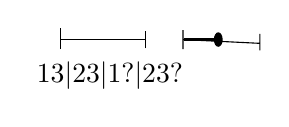
\begin{tikzpicture}[scale=.8]\draw (0,0)--(1.35,0) (0,-.15)--(0,.18) (1.35,-.14)--(1.35,.13); \node at (.78,-.57){$\unsure{13|23|1?|23?}$}; \draw(1.94,0)--(3.16,-.06) (1.94,-.15)--(1.94,.15) (3.16,-.17)--(3.16,.09); \draw[very thick](1.95,0)--(2.5,0);\fill(2.5,0)ellipse(.07 and .115);\end{tikzpicture}}

% 17–20, left repeated triangle
\diagram{\begin{tikzcd}[ampersand replacement=\&,column sep=0.4em,row sep=small]
\&\& D_{012}\arrow[dl,dash]\arrow[d,very thick,dash]\arrow[dr,"\text{épi}",dash]\\
\&D_{01}\arrow[dl]\arrow[dr,"\text{épi}"']\&D_{02}\arrow[dll,dash]\arrow[drr,dash]\&D_{12}\arrow[dl,dash]\arrow[dr,"\text{épi}",dash]\\
 D_0\&\&D_1\&\&D_2
\end{tikzcd}}

% 17–21, right-hand criterion
$D_\sigma\unsure{-|\to}D_{\sigma'}$ épi \uline{si} $\sigma'\subset\sigma$ est segment final de $\sigma$ i.e. $\sigma=\sigma''\cup\sigma'$ avec $\sigma''<\sigma'$

% 17, isolated mark above the lower diagram
$\unsure{7|\urcorner}$

% 19–24, large diagram
\diagram{\begin{tikzcd}[ampersand replacement=\&,row sep=small,column sep=0.05em]
\&\&\&\&\&\&D_{0123}\arrow[dlll]\arrow[d]\arrow[dr,very thick]\\
\&\&\&D_{013}\arrow[ddll,bend right=20]\arrow[dr]\arrow[drr,very thick]\&\&\&D_{023}\arrow[dll,dashed]\arrow[dr,very thick]\&D_{123}\arrow[dll]\arrow[d,very thick]\\
\&\&D_{012}\arrow[dl,dashed]\arrow[d]\arrow[dr,very thick,"\text{épi}"]\arrow[dd,bend left=65]\arrow[rr,dash]\&\&D_{03}\arrow[ddr,very thick]\&D_{13}\arrow[dd,very thick]\&\&D_{23}\arrow[ddll,very thick]\\
\&D_{01}\arrow[dl]\arrow[d,very thick]\&D_{02}\arrow[dll,dashed]\arrow[d,very thick]\&D_{12}\arrow[dll,dashed]\arrow[dl,very thick,"\text{épi}"]\\
D_0\&D_1\&D_2\&\&\&D_3
\end{tikzcd}}

% 25–28, two columns at foot
\[
\begin{aligned}
D_{01}&\mathbin{-}D_1 &D_{013}&\mathbin{-}D_{13}\\
D_{012}&\to D_{12} &D_{0123}&\mathbin{-}D_{123}\\
D_{12}&\mathbin{-}D_2 &D_{123}&\mathbin{-}D_{23}\\
D_{02}&\mathbin{-}D_2 &D_{23}&\mathbin{-}D_3
\end{aligned}
\]

% bottom right, ruled wedge with indices
\figure{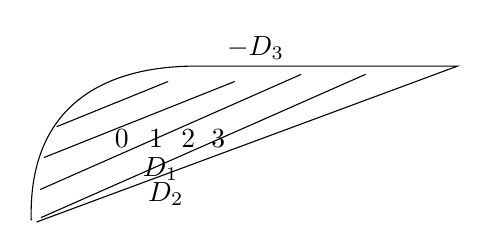
\begin{tikzpicture}[x=.95cm,y=.7cm]\draw (0,0)..controls (-.04,2) and (.9,2.8)..(2.21,2.8)--(5.7,2.8)--(.07,-.03); \draw (.34,1.7)--(1.83,2.52) (.17,1.14)--(2.72,2.52) (.12,.56)--(3.61,2.65) (.13,.05)--(4.47,2.65); \node at (3,3.12){$-D_3$}; \foreach \x/\v in {1.21/0,1.67/1,2.1/2,2.5/3}{\node at (\x,1.48){$\v$};} \node at (1.73,.93){$D_1$}; \node at (1.8,.48){$D_2$};\end{tikzpicture}}

% bottom, numerical working
\[
\begin{aligned}
&1\quad 1+1\quad 1+2+\\[-1pt]
&\hspace{3em}\shortparallel\\[-1pt]
 n_i&=\sum_{j<i}n_j+1\qquad 2
\end{aligned}
\]

% lower left
% archive sheet number: 11
\scanpage{13}

% 1, upper left
1) \quad $F_0$

% 2, first diagram
\diagram{\begin{tikzcd}[ampersand replacement=\&,column sep=small,row sep=small]
\&R_1\arrow[dl]\arrow[dr,"\text{épi}"]\\
2)\ F_0\&\&F_1
\end{tikzcd}}

% 3, cancelled first attempt
\diagram{\begin{tikzcd}[ampersand replacement=\&,column sep=tiny,row sep=tiny,execute at end picture={\draw[thick] (\tikzcdmatrixname-1-2.west) -- (\tikzcdmatrixname-2-1.west) -- (\tikzcdmatrixname-1-2.east) -- (\tikzcdmatrixname-3-1.east) -- (\tikzcdmatrixname-2-3.north) -- (\tikzcdmatrixname-3-3.west);}]
\&\deleted{R'_1}\arrow[dl]\arrow[dr,"\deleted{\text{épi}}"]\\
3)\ \deleted{F'_0}\arrow[d]\&\deleted{R_1}\arrow[dl]\arrow[dr,"\deleted{\text{épi}}"]\&\deleted{F'_1}\arrow[d]\\
F_0\&\&F_1\&F_2
\end{tikzcd}}

% 3, second drawing beside crossed version
\diagram{\begin{tikzcd}[ampersand replacement=\&,row sep=small,column sep=small]
\& R'_1\arrow[dl,very thick]\arrow[dr,two heads]\arrow[dd,very thick]\arrow[dddrr,dashed]\\
F'_0\arrow[dd,very thick]\arrow[ddrrr,dashed]\&\& F'_1\arrow[dd,very thick]\arrow[ddr]\\
\&R_1\arrow[dl]\arrow[dr,two heads]\\
F_0\&\&F_1\&F_2
\end{tikzcd}}

% top right, decomposition and list
décomposition cellulaire \deleted{drapeaux} \inserted{correspond : l'ens} \deleted{\unsure{complexe simplicial|quasi-simplicial} sommets $=F_0\amalg F_1$} ordonné des drapeaux
\[
\begin{aligned}
\text{type }0 &:F_0\\
\text{type }1 &:F_1\\
\text{type }(0,1)&:R_1
\end{aligned}
\]

% top right, marked points and loops
\figure{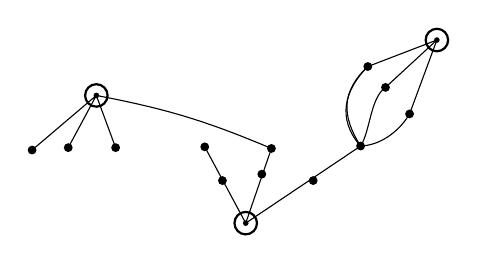
\begin{tikzpicture}[x=1.02cm,y=1.02cm]
\coordinate (a) at (.8,1.25); \coordinate (b) at (2.66,-.34); \coordinate (c) at (4.09,.62); \coordinate (d) at (5.04,1.94);
\draw (0,.57)--(a)--(.45,.6) (a)--(1.04,.6) (a) to[bend left=6](2.98,.59)--(b)--(2.15,.61) (b)--(c);
\draw (c)..controls (3.79,.96) and (3.89,1.32)..(4.18,1.61)--(d);
\draw (c)..controls (3.85,1) and (3.85,1.3)..(4.18,1.61);
\draw (c)..controls (4.21,.8) and (4.21,1.22)..(4.4,1.35)--(d);
\draw (c)..controls (4.36,.63) and (4.59,.83)..(4.7,1.02)--(d);
\foreach \p in {(0,.57),(.45,.6),(1.04,.6),(2.15,.61),(2.37,.19),(2.86,.27),(2.98,.59),(3.5,.19),(c),(4.18,1.61),(4.4,1.35),(4.7,1.02)}{\fill \p circle(.055);}
\foreach \p in {a,b,d}{\draw[thick](\p)circle(.14); \fill(\p)circle(.035);}
\end{tikzpicture}}

% 4, below left
4) \qquad $F_0$

% 4, below the isolated F
\diagram{\begin{tikzcd}[ampersand replacement=\&,row sep=small,column sep=small]
\& R'_1\arrow[dl,very thick]\arrow[dr,two heads]\arrow[dd,very thick]\arrow[dddrr,dashed]\\
F'_0\arrow[dd,dash]\arrow[ddrrr,dashed]\&\& F'_1\arrow[dd,very thick]\arrow[ddr]\\
\&R_1\arrow[dl]\arrow[dr,two heads]\\
F_0\&\&F_1\&AF_2
\end{tikzcd}}

% lower left, initial categories
$\deleted{C_0=\unsure{\mathrm{Ens}_f|\mathrm{Ens} f}}$

$C_1={}$

% lower half, definition of family category
$\Phi(C)={}$ Catégorie des \deleted{\unsure{couples|triples}} \deleted{\unsure{$I,$}} \inserted{familles finies} $\{(f_i)_{i\in I}\}$ de morphismes de $C$ de \unsure{$=$|m\textsuperscript{e}} but \deleted{\unsure{$I$, ens. fin.}}

% below definition, induced functor
Un foncteur $C\xrightarrow{\unsure{r|\varphi}}(\mathrm{Top}\ \deleted{\unsure{isotop.}})$ implique un foncteur
\[
 \begin{aligned}
 \Phi(C)&\xrightarrow{\deleted{\unsure{\varphi}}\Phi(r)}\mathrm{Top}\\
 (X_i\overset{\unsure{f_i}}{\to} X)_{i\in I}&\longmapsto
 \coprod_i\underbrace{\operatorname{cône}}_{\mathord{\hookrightarrow}}\deleted{\unsure{F|\varphi}}r(X_i)
 \underset{\coprod\Phi(X_i)}{\amalg}r(X)
 \end{aligned}
\]

% near bottom, finiteness
Si les $r(f)$ $(f\in\mathrm{Fl}(C))$ sont finis, de $=$ les $\Phi(r)(f)$ $(f\in\mathrm{Fl}(\Phi(C)))$

% near bottom, faithfulness
Si $r$ est \deleted{\unsure{pl.}} fidèle (resp. pl. fidèle) $\Phi(r)$ idem vers les espaces top. filtrés \uline{mod isotopie}\ldots.

% last line
\[
 \Phi(\Phi(C))\longrightarrow\mathrm{Top}
\]

% lower left
% archive sheet number: 12
\scanpage{14}

% 1–3, paratriangulations and paracartes
\deleted{\unsure{espaces}} paratriangulations

paracartes : foncteurs $\unsure{\mathscr P_f^*|\mathscr P_f^\wedge|\mathfrak P_f^*}(\mathbb N)\xrightarrow{D}(\mathrm{Ens})$ tels que $\sigma'\subset\sigma$ \inserted{segment final} $\Rightarrow D(\sigma)\to D(\sigma')$ épi

% 4–6, n-equidimensional case
paracartes $n$-équidimensionnelles : $\big\{D(\sigma)\mathbin{-}D(\sigma')$ \unsure{tjs|bij.} épi si \deleted{$\operatorname{Sup}\sigma=\operatorname{Sup}\sigma'$} $\sigma\subset\sigma'\subset\Delta_n$, et $D(\{i\})=0$ si $i>n$.

% 7–9, strata
paracartes à \deleted{\unsure{filtra}} strates équidimensionnelles : $D(\unsure{\Delta_i|\Delta_n|\sigma})\mathbin{-}D(\sigma')$ épi si $\operatorname{Sup}\sigma=\operatorname{Sup}\sigma'$

i.e. $D([0,i])\to D(\sigma)$ épi si $i=\operatorname{Sup}\sigma$

% 10–13, special paracartes
\uline{paracartes} \uline{spéciales} \quad $\left\{\begin{aligned}
 &\text{\unsure{précédentes|bicellules|les cellules} : équidim}\\
 &\forall\ \deleted{i\ \text{\unsure{tel que}}\ D(\{i\})\ne\varnothing,\ \text{\unsure{le}}}\ \inserted{0\leq j\leq i}\\
 &D(0,\ldots,j-1,j+1,\ldots i)\longleftarrow D(0,\ldots,i)\\
 &\hspace{5em}\text{\uline{de degré 2}}
 \end{aligned}\right.$

% 11–13, small examples at left
\diagram{\begin{tikzcd}[ampersand replacement=\&,column sep=small,row sep=tiny]
D_{01}\arrow[d]\&\&D_{012}\arrow[dl]\arrow[dr]\\
D_1\&D_{12}\&\&D_{02}
\end{tikzcd}}

% 14–16, question
\uline{Question} : \unsure{a-t-on|t-on} $D(\ldots j-1,j\unsure{+|,}j+1\ldots)\mathbin{-}D(\deleted{\unsure{j\ldots}}j-1,j+1,\ldots)$ tjs de degré 2 ?? p. ex $D_{123}\to D_{13}$ degré 2\ldots

% 17–20, groups and reconstruction
d'où groupe $G_{i-1}$ engendré par $\sigma_0\ldots\sigma_{i-1}$ opérant sur $\unsure{R|\mathscr R}_i$
\[
 \underset{\shortparallel}{R_i}\qquad D(0,\ldots,i)
\]
On veut condition assurant qu'on \uline{récupère} les \deleted{\unsure{g}} $D(i_0,i_1\ldots i_p)$ \deleted{\unsure{$g$}} via $(R_i,G_{i-1})$ et les applications $R_{i+1}\mathbin{-}R_i\mathbin{-}\ldots$

% lower left
% archive sheet number: 13
\scanpage{16}

% 1–3, definition
Un ens ordonné \inserted{$D$} est appelé ``géométrie de drapeaux'' si pour tout $d\in D$, l'ens. \deleted{\unsure{dessous|dessiné|ordonné}} \inserted{\unsure{induit|initial}} $D(d)=\{d'\in D\mid d'\leq d\}$ a la structure d'un ``simplexe ordonné'' i.e. est isomorphe à $\unsure{\mathscr P^*|\mathcal P^*|\mathfrak P^*}(I_d)$,

% 2–3, upper right, directed to the power set
\margin{parties finies $\ne\varnothing$}

% 3–4, outer left
% slanted
\margin{\uline{NB} on aura donc $I_d\ne\varnothing$}

% 4–8, minimal elements and length
avec l'inclusion --- où $I_d$ peut s'identifier à l'ens des él. minimaux de $D(d)$, ou encore : la partie de l'ens $\Phi\unsure{=|.}D(\underline{1})$ des él. minimaux de $D$ (``drapeaux de longueur 1 --- NB $\operatorname{card}(I_d)$ s'appellera ``longueur'' du drapeau $d$).

% 8–11, antifacteur
Pour toute partie finie $\sigma$ de $\Phi$, soit $D(\sigma)$ l'ens des $d\in D$ tels que $\deleted{\unsure{\sigma\subset}}I_d\deleted{\unsure{\ni}}=\sigma$, on trouve un antifoncteur
\[
 (\text{parties finies \inserted{$\ne\varnothing$} de }\Phi)^o\xrightarrow{D}(\mathrm{Ens})\qquad
 \text{tel que }\operatorname{card}D(\{i\})=1\quad\forall i\in\Phi
\]

% 12–14, reconstruction
dont la connaissance permet de reconstituer $D_{\unsure{*|{}}}$ comme
\[
 D_{\unsure{*|{}}}\simeq\coprod_{\sigma\in\mathscr P_f^*(\Phi)}D(\sigma)
\]
avec la relation d'ordre évidente. Ainsi

% 15–18, equivalence
\[
\begin{aligned}
\left\{\begin{array}{l}\text{géométrie de drapeaux}\\\text{(ens. ordonné \unsure{abs.|avec|ainsi})}\end{array}\right.
 &\Longleftrightarrow \begin{array}{l}
 \text{Couple }(\Phi,D)\text{ d'un ens}\\
 \Phi\text{ et d'un foncteur}\\
 \underline{\mathscr P_f^*}(\Phi)^o\mathbin{-}(\mathrm{Ens})\\
 \text{tel que }\operatorname{card}D(\{i\})=\unsure{4|1}\quad\forall i\in\unsure{I|\Phi}
 \end{array}
\end{aligned}
\]

% 17–19, lower left of equivalence
\margin{\uline{NB} $\Phi$ est tjrs l'ens des sommets d'une maquette simpliciale, mais bien sûr $D$ n'est pas déterminé par celle-ci\ldots}

% 19–20, strictness
\uline{NB} Pour que dans $D$ on ait $\forall d\in D$
\[
 d=\mathop{\rm Sup}_{i\in I_d}i
\]

% 19–20, right of supremum formula
\margin{géom de drapeaux stricte}

% 21–24, subsets
il f. et s. que $D$ soit isomorphe à un ens des parties finies \inserted{$\ne\varnothing$} de $\Phi$ avec l'inclusion (contenant les parties finies ponctuelles et contenant, avec tout ens, les ens $\ne\varnothing$ plus petits). On trouve ainsi

% 25, correspondence
\[
 \left(\begin{array}{c}\text{géom. de drapeaux}\\\text{stricte}\end{array}\right)
 \Longleftrightarrow
 \left(\begin{array}{c}\text{maquettes}\\\text{simpliciales}\end{array}\right)
\]

% 26–28, functor formulation
En termes du foncteur $D:\mathscr P_f^{\unsure{\triangle|*}}(\Phi)^o\mathbin{-}(\mathrm{Ens})$, celà signifie que $D$ est \deleted{le} \inserted{\unsure{sous|isom. à un|un sous-}} foncteur \deleted{\unsure{prenant}} \inserted{du foncteur} \inserted{final i.e.} \deleted{qui \unsure{en chaque} $\sigma$, \unsure{a pour}} $\forall\sigma,$ $\operatorname{card}D(\sigma)\leq1$ i.e. $\operatorname{card}D(\sigma)\in\{0,1\}$

% lower left
% archive sheet number: 15
\scanpage{17}

% 1–3, opening and functor
\inserted{Soit $I$ un ens et} Supposons qu'on ait un foncteur
\[
 \underline{\unsure{\mathscr P_f^\wedge|\mathscr P_f^*|\mathfrak P_f^*}}(I)^o\xrightarrow{D'}(\mathrm{Ens})
\]

% 4–7, flag geometry
sans condition de la forme $\operatorname{card}D(\{i\})=1$ $\unsure{\forall i\in I|\text{lorsque}}\unsure{)|{}}$. On peut néanmoins lui associer une géom. de drapeaux \deleted{dont l'ens des}
\[
 D=\coprod_{\sigma\in\mathscr P_f^*(I)}D'(\sigma)
\]

% 8–11, minimal elements and map
dont l'ens des él. minimaux est
\[
 \Phi=\coprod_{\substack{\deleted{\unsure{\sigma\in\mathscr P_f^*}}\\\inserted{i\in I}}}D'(\{i\})
\]
On a donc une application
\[
 \Phi\xrightarrow{\delta}I
\]

% 12–16, restriction
(application ``dim'' \deleted{\unsure{$\delta$}} dans les cas qui nous intéressent) ayant la propriété que pour tout $d\in D$, la restriction \deleted{$\delta|I_d:\unsure{d\ldots}$}
\[
 \delta\mid I_d\unsure{.|{}}\ :\ I_d\longrightarrow I
\]
est injective.

% 16–20, converse
Inversement, étant donné une géom de drapeaux $D$ et une application $\delta$ de $\Phi=D(1)$ (ens des él. minimaux de $D$) dans un ens $I$, satisfaisant la condition précédente, on lui associe un foncteur

% 21–23, associated functor
\[
\begin{aligned}
 &D':\underline{\mathscr P_f^{\unsure{+|*}}}(I)\to(\mathrm{Ens})\qquad\text{par}\\
 &D'(\sigma)=\coprod_{\substack{\sigma'\in\mathscr P_f^*(\unsure{I|\Phi})\\\text{t.q. }\delta|\sigma':\sigma'\unsure{\simeq|\overset{\sim}{\to}}\sigma}}D(\sigma')
\end{aligned}
\]

% 24–25, recovery
et on voit que $(D,I,\delta)$ se réconstitue à partir de $(I,D')$. \unsure{Donc|Bref}

% lower left
% archive sheet number: 16
\scanpage{18}

% 1–4, equivalence at head
\diagram{\begin{tikzcd}[ampersand replacement=\&,column sep=large]
\left.\begin{gathered}
 \text{géom. de drapeaux } D\\[-2pt]
 {}+\text{ ``\deleted{\unsure{application}}\inserted{fonction} dimension''}\\
 \delta:\underset{\substack{\downarrow\\\text{él. min.}}}{\Phi}\longrightarrow I
\end{gathered}\right| \arrow[r,Leftrightarrow] \&
\left|\ \text{foncteur }D'/\underline{\unsure{\mathscr P_f^*|\mathcal P_f^*|\mathfrak P_f^*}}(I)^o\to(\mathrm{Ens})\right.
\end{tikzcd}}

% 3–6, below right-hand member and across middle
\margin{\uline{NB} Posant $I_0=\{i\in I\mid D'(\{i\})\ne\varnothing\}$ on a sur $I_0$ une structure de \unsure{maquette simpl.|m. géométr. simpl.|ens. quasi-simpl.}, ayant comme simplexes les $\sigma$ tels que $D'(\sigma)\ne\varnothing$. \inserted{(NB $I_0=\delta(\Phi)$).}}

% 7–9, case of the natural numbers
Le cas qui nous intéresse plus particulièrement est le cas
\[
 I=\mathbb N
\]

% 10–14, dimension
auquel cas $\delta$ prend le nom de fonction dimension \deleted{\unsure{$\Phi/I$}} Et $\sup_{\overline{\mathbb R}}\delta(I)$ \deleted{\unsure{prend le nom}}\inserted{s'appelle} la dimension de la géom. de drapeaux $D$ \deleted{\unsure{avec sa dimension}}\inserted{(munie de sa} fonction dimension). Si celle-ci est finie, soit $n$, il y a souvent avantage à remplacer $\mathbb N$ par $[0,n]_{\mathbb N}$.

% 15–20, general construction
Plus gén., \inserted{(pour une géom. de drapeaux $D$ donnée)} supposons donnée une loi qui associe à chaque \deleted{partie} simplexe $\sigma\subset\underline{\Phi}$ (i.e. $\sigma\in\mathscr P_f^*(\Phi)$ de la forme $I_d$) un \uline{ordre total} sur $\sigma$, de façon que ces ordres totaux s'induisent mutuellement

% 20–27, orders and preorders
[ce qui est le cas pour les ordres totaux induits par un $\delta:\underline{\Phi}\to I$ si $I$ lui-m\unsure{e} est tot. ordonné, ou muni d'un \inserted{pré}ordre \deleted{\unsure{induisant}} pour lequel les simplexes de $I$ sont tot. ord...) mais cela revient à prendre sur $I$ le \inserted{pré}ordre image inverse...] Alors, posant pour $n\in\mathbb N$ ($n\geq0$)

% 28–30, D[n]
\[
 \begin{aligned}
 D[n]&=\{d\in D\mid\operatorname{card}I_d=n+1\}\\
 &=\coprod_{\sigma\in\mathscr P_{\unsure{f\,n+1|n+1}}(\Phi)}D(\sigma)\\
 &\left(\underset{\text{ou \unsure{s'ident.|seulement|aussi}}}{=}\
 \coprod_{\sigma\in\mathscr P_{f\,n+1}(I)}D'(\sigma)\right)
 \end{aligned}
\]

% lower left
% archive sheet number: 17
